\documentclass[12pt]{article}

% basic package list
\usepackage[T1]{fontenc}
\usepackage{fontspec}
\defaultfontfeatures{Mapping=tex-text}
\usepackage[margin=25mm]{geometry}
\usepackage{amsmath}
\usepackage{amsfonts}
\usepackage{amssymb}
\usepackage{graphicx}
%\setmainfont{???}

% other packages
\usepackage{xunicode}
\usepackage{xltxtra}
\usepackage{hyperref}         % hyperlinks
\usepackage{booktabs}         % professional-quality tables
\usepackage{indentfirst}      % to indent section first paragraph
\usepackage{url}              % simple URL typesetting
\usepackage{natbib}
\usepackage[modulo]{lineno}
\usepackage{sectsty}          % to change section font size
\usepackage{mathtools}

% set additional parameters
\setcitestyle{authoryear,open={(},close={)}}
\graphicspath {{Figures/}}

\sectionfont{\fontsize{18}{22}\selectfont}
\subsectionfont{\fontsize{16}{19}\selectfont}

\title{Supporting Information for: Joint inference of adaptive and demographic history from temporal population genomic data}
\author{Vitor A. C. Pavinato$^1$, Stéphane de Mita$^2$, Jean-Michel Marin$^3$, \\
			Miguel Navascués$^1$$^*$}
\font\myfont=cmr12 at 10pt
\date{{\myfont %
    $^1$UMR Centre de Biologie pour la Gestion des Populations, INRA, France\\%
    $^2$UMR Interactions Arbres-Microorganismes, INRA, France \\%
    $^3$UMR Institut Montpelliérain Alexander Grothendieck, Université de Montpellier, France\\%
    $^*$corresponding author: miguel.navascues@inra.fr\\[2ex]%
    }
    \today    
}
\begin{document}
\maketitle
\newpage
\section*{S1 Supplementary Methods}

\subsection*{S1.1 Model}

\begin{figure}[ht]
  \centering
  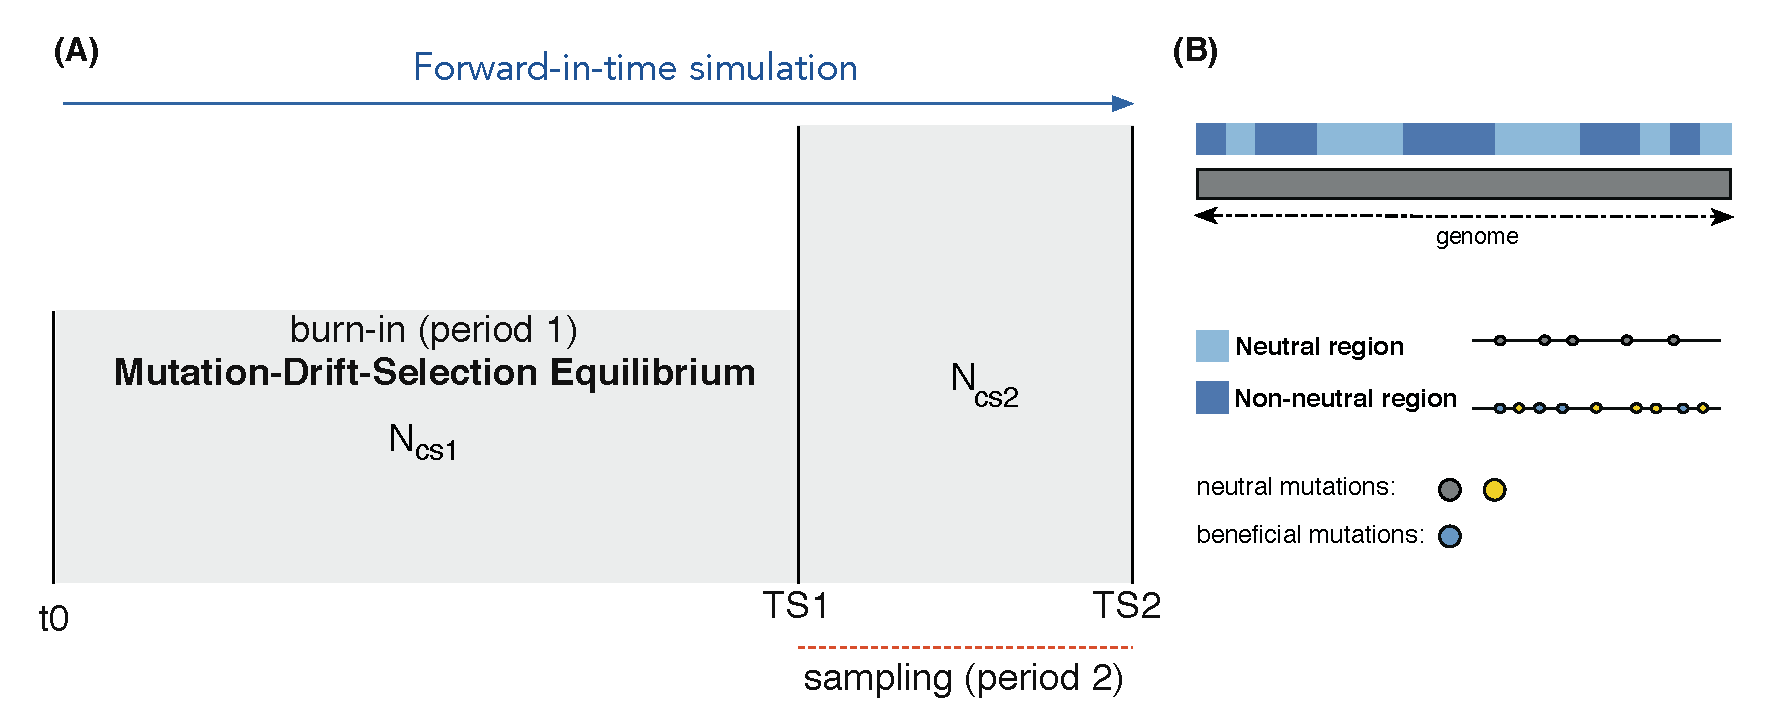
\includegraphics[width=0.9\textwidth]{model.pdf}
  \label{fig:figS1}
  \caption{A schematic representation of the model used to simulate temporal population genomics data. \textbf{(A)} the population model. The model was composed by two periods: 1) the burn-in period and 2) the sampling period. Both periods had independent prior for the parameter that controlled the population census size: $N_{CS_{1}}$ and $N_{CS_{2}}$. The interest were in the selection dynamics of the sampling period. In order to calculate the summary statistics, we sampled the genotypic data in to time-points TS1 and TS2 apart $\tau$ generations. \textbf{(B)} the genome model. The genome of each diploid individual was divided in fragments that were defined either neutral or non-neutral. The proportion of non-neutral regions was defined by $P_{R}$ and the probability of a beneficial mutation to arise in a non-neutral regions was defined by $P_{B}$. The compound parameter $P_{S} = P_{R}*P_{B}$ defined the proportion of selection mutation that might arise in a simulation}
\end{figure}

\subsection*{S1.2 List of summary statistics}

List of the summary statistic used to produced the reference table for the evaluation of ABC-RF (SNP and windowed-based summary statistics):
\begin{enumerate}
	\item Locus-specific summary statistics - SNP-based:
    \begin{enumerate}
    	\item Expected heterozygosity - $H_E$;
        \item Jost's $D$ \citep{Jost:2008cs,Jost:2009hn} - $Dj$;
        \item Weir and Cockerham's $F_{ST}$ \citep{Weir:1984dx} - $WC_{ST}$;
    \end{enumerate}
    \item Locus-specific summary statistics - window-based:
    \begin{enumerate}
        \item Number of polymorphic sites $S$;
        \item Nucleotide diversity $\pi$ \citep{Nei:1979uk};
        \item Watterson's 4Nu estimator \citep{Watterson:1975bh} - $thetaW$;
        \item Tajima's D \citep{Tajima:1989un} - $TjD$;
        \item Net distance between populations $Da$;
        \item Rozas et al.'s $ZZ$ \citep{Rozas:2001wc};
        \item Average of $R^2$ over all pairwise comparisons $Z_{nS}$ \citep{Kelly:1997uja}; 
    \end{enumerate}
    \item Global summary statistics:
    \begin{enumerate}
        \item All summary statistics enumerated above;
        \item binned Joint Site-frequency spectrum $SFS$ \citep{Ewing:2016gv};
        \item mean, variance, kurtosis, skewness and the 5\% and 95\% quantiles of all intra-locus summary statistics calculated above;
    \end{enumerate}
\end{enumerate}

\bibliographystyle{apalike}
\bibliography{references}
\end{document}

\cit